\chapter{Проектирование системы дистрибуции программных модулей}
\label{cha:design}

Проектирование системы дистрибуции программных модулей - это сложная задача, ставка при которой делается не только на функциональность, но и на безопасность. 

\section{Выбор архитектуры системы}

Современная разработка ПО основывается на двух основных типах архитектуры: монолитной и микросервисной. Давайте кратко рассмотрим каждый из этих типов. 

Монолитная архитектура представляет собой классическую модель подхода к программному обеспечению, где используется один самостоятельный модуль, функционирующий отдельно от других приложений. Именно поэтому ее и называют "монолитной". Все фрагменты кода и бизнес-функции в такой архитектуре объединены в одной области \cite{arch:monovsmicro}.

\begin{figure}
  \centering
  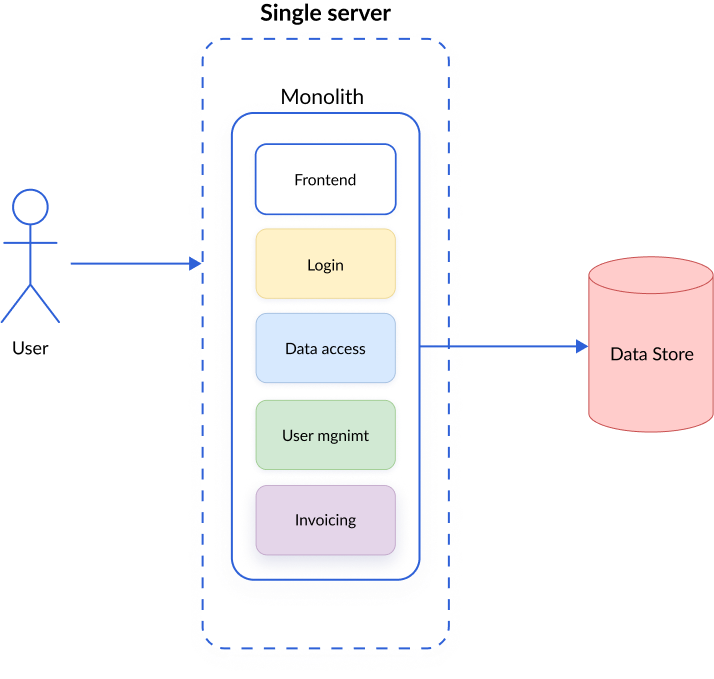
\includegraphics[width=.7\textwidth]{graphics/img/mono.png}
  \caption{Пример монолитной архитектуры}
  \label{fig:mono}
\end{figure}


Микросервисная архитектура - это разделение архитектуры на множество независимо функционирующих служб. Каждая из этих служб имеет свою бизнес-логику и систему управления базами данных (СУБД), служащую определенной цели. Оба эти типа архитектур стоит рассмотреть в контексте сравнения.

\begin{figure}
  \centering
  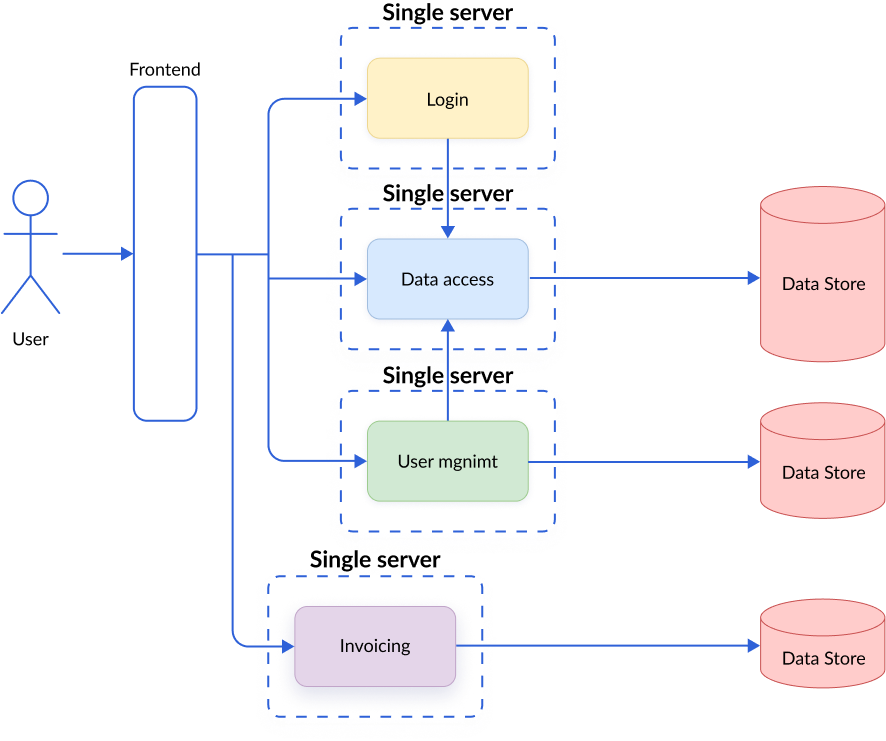
\includegraphics[width=.9\textwidth]{graphics/img/micro.png}
  \caption{Пример микросервисной архитектуры}
  \label{fig:micro}
\end{figure}

Среди недостатков монолитной архитектуры можно выделить плохую масштабируемость, трудность внедрения новых модулей и проблемы при обновлении технологий, так как это может затронуть весь проект, к тому же есть и проблемы с отказоустойчивостью и трудностью в горизонтальной масштабируемости. Однако она проще в развертывании, разработке, тестировании и отладке, чем микросервисная \cite{arch:monovsmicro}. 

Микросервисная архитектура обладает гибкостью: каждая команда может разрабатывать и разворачивать свой сервис независимо, что ускоряет сроки реализации проектов и позволяет выбирать технологии согласно предпочтениям команды. Отказоустойчивость в данном случае - тоже немаловажный плюс, поскольку при сбое одного микросервиса функциональность приложения страдает лишь частично. Недостатками же можно считать большие временные затраты при разрастании приложения и сложность отладки и координации между разными командами.

Текущий проект предполагает высокую нагрузку, переносимость и отказоустойчивость. В связи с этим было принято решение о применении микросервисной архитектуры, которую неспроста выбирают и многие существующие системы, поскольку в условиях повышенных требований эксплуатации требуется более гибкая система.

\section{Функциональные возможности системы}

Определенные требования приводят нас к функциональным возможностям проектируемой системы:

\subsection{Серверная часть}

Серверная часть системы должна обеспечить следущие функции:

\begin{enumerate}
    \item Загрузка на сервер, отправка пакета (модуля) с сервера.
    \item Управление зависимостями модулей.
    \item Система версий модулей.
    \item Информирование о модулях и их безопасности.
    \item Аутентификация и авторизация на основе JWT.
    \item Реализация открытого API.
    \item Система блокировки и защиты особо критических модулей.
\end{enumerate}

\Define{API}{Application Programming Interface ""--- представляет собой набор правил и инструкций, согласно которым различные программы и сервисы могут общаться между собой. Эти правила определяют, как данные и функциональность могут быть переданы от одной программы к другой, как они могут взаимодействовать и обмениваться информацией}

\subsection{Клиентская часть}

Клиентская часть системы должна иметь следующую функциональность:

\begin{enumerate}
    \item предоставление простого и понятный интерфейса через CLI.
    \item конфигурирование клиентской части.
    \item управление установленными модулями, включая загрузку, обновление и удаление.
    \item информирование о модулях и их безопасности.
\end{enumerate}

\section{Микросервис авторизации и аутентификации}

В рамках данной работы предполагается разработка микросервиса авторизации для системы, который будет выполнять следующие функции:

\begin{enumerate}
    \item осуществлять регистрацию пользователя.
    \item производить механизмы аутентификации и авторизации пользователя.
    \item обслуживать систему сессий через JWT.
    \item предоставлять систему прав у пользователей.
\end{enumerate}

\begin{figure}
  \centering
  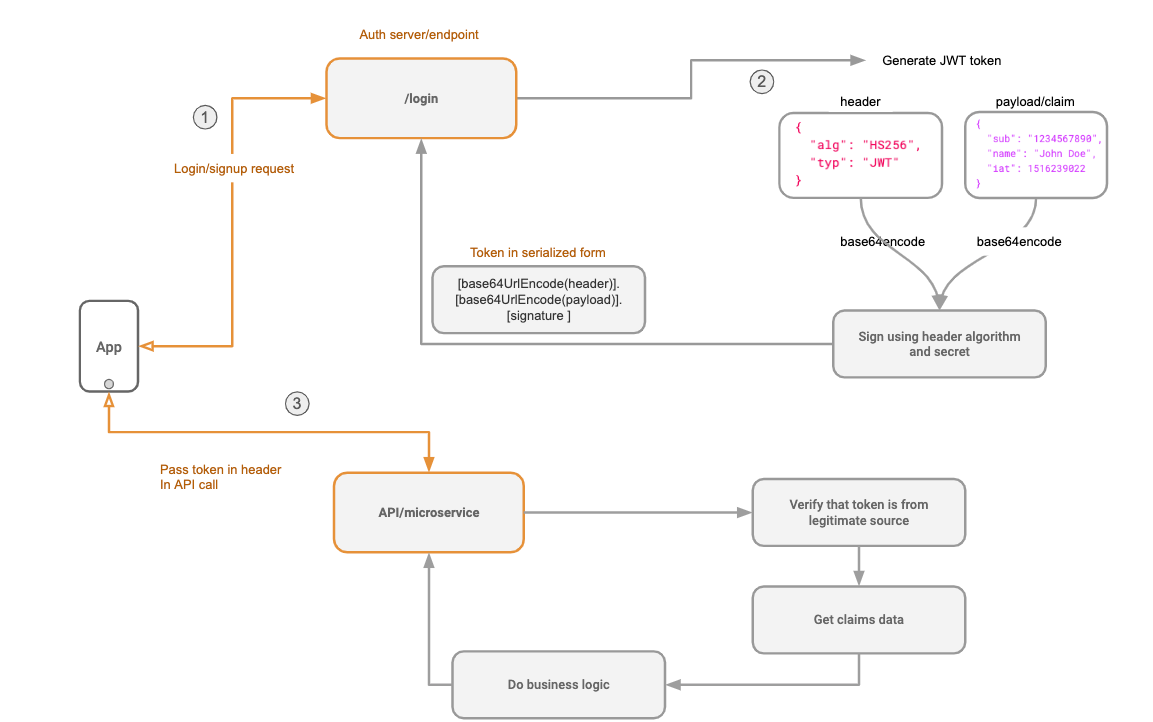
\includegraphics[width=0.8\textwidth]{graphics/img/jwt.png}
  \caption{Функционирование JWT в связке клиент-сервер}
  \label{fig:jwt}
\end{figure}

\Define{JWT}{JSON Web Token ""--- универсальное средство формирования токенов доступа, основанный на надежном и широкораспространенном формате JSON с учетом открытого стандарта RFC 7519, он стал одним из наиболее эффективных и безопасных способов обеспечения эффективной передачи информации между устройствами и серверами в кодированном виде}

\section{API Gateway}
Для полноценного функционирования и получения доступка к микросервисам из любой точки Интернета, необходима единая точка входа, называемая API Gatawey, которым будет выступать прокси сервер nginx с модулем поддержки JWT \cite{arch:api}. 

Основные функции точки входа:
\begin{enumerate}
    \item проксировать на необходимые микросервисы;
    \item балансировать нагрузки на запущенные микросервисы;
    \item проверять и производить прочие действия с JWT;
    \item обеспечивать реализацию всех современных стандартов безопасности (CORS и прочие механизмы);
\end{enumerate}

\Define{nginx}{это HTTP-сервер и обратный прокси-сервер, почтовый прокси-сервер, а также TCP/UDP прокси-сервер общего назначения, изначально написанный Игорем Сысоевым}

\Define{CORS-заголовки}{(Cross-Origin Resource Sharing) ""--- это механизм веб-безопасности, который позволяет браузеру загружать данные из стороннего интернет-источника.}

\Define{API Gatawey}{шлюз для API, который упрощает управление и делает доступными для клиентов.}

Таким образом, только API Gateway и микросервис авторизации имеют доступ к единому хранилищу, где располагается секретный ключ, используемый для подписи JWT, что повышает безопасность системы в целом. Для предовращения и снижения риска компроментации, ключ рекомендуется менять раз в месяц. 

\section{Микросервис управления пакетами}

Микросервис управления модулями является основным и включает в себя ряд функций. 

\subsection{Базовый функционал}
Сервис обеспечивает добавление новых модулей, управление их распределением и поиск по модулям в соответствии с запросами пользователя.

\subsection{Система зависимостей}
Сервис предоставляет возможность модулям иметь систему зависимостей, что позволяет создавать модульные приложения и пакеты.

\subsection{Блокировка, поиск уязвимостей и удаление модулей}
Ключевую роль в функционале микросервиса играет возможность блокировки модулей, что является важным средством контроля доступа. Кроме того, микросервис может производить поиск и устранение уязвимостей в модулях, что особенно важно с точки зрения безопасности системы.

\subsection{Информирование}
Функция информирования обеспечивает прозрачность и контроль над процессами управления модулями. С помощью неё пользователи могут получать обновленную информацию о статусе операций и о состоянии модулей.

\section{CDN}

\Define{CDN}{Content Delivery Network ""--- это сеть распределенных серверов, которые эффективно передают контент пользователям, основываясь на их географическом положении, источнике контента и сервере с оригинальным содержимым}

В контексте проектирования системы, CDN обеспечивает надежную, высокоскоростную и эффективную доставку модулей от сервера к клиенту. Благодаря CDN, пакеты кода или модулей могут быть быстро и эффективно переданы пользователям независимо от их географического расположения.

\begin{figure}
  \centering
  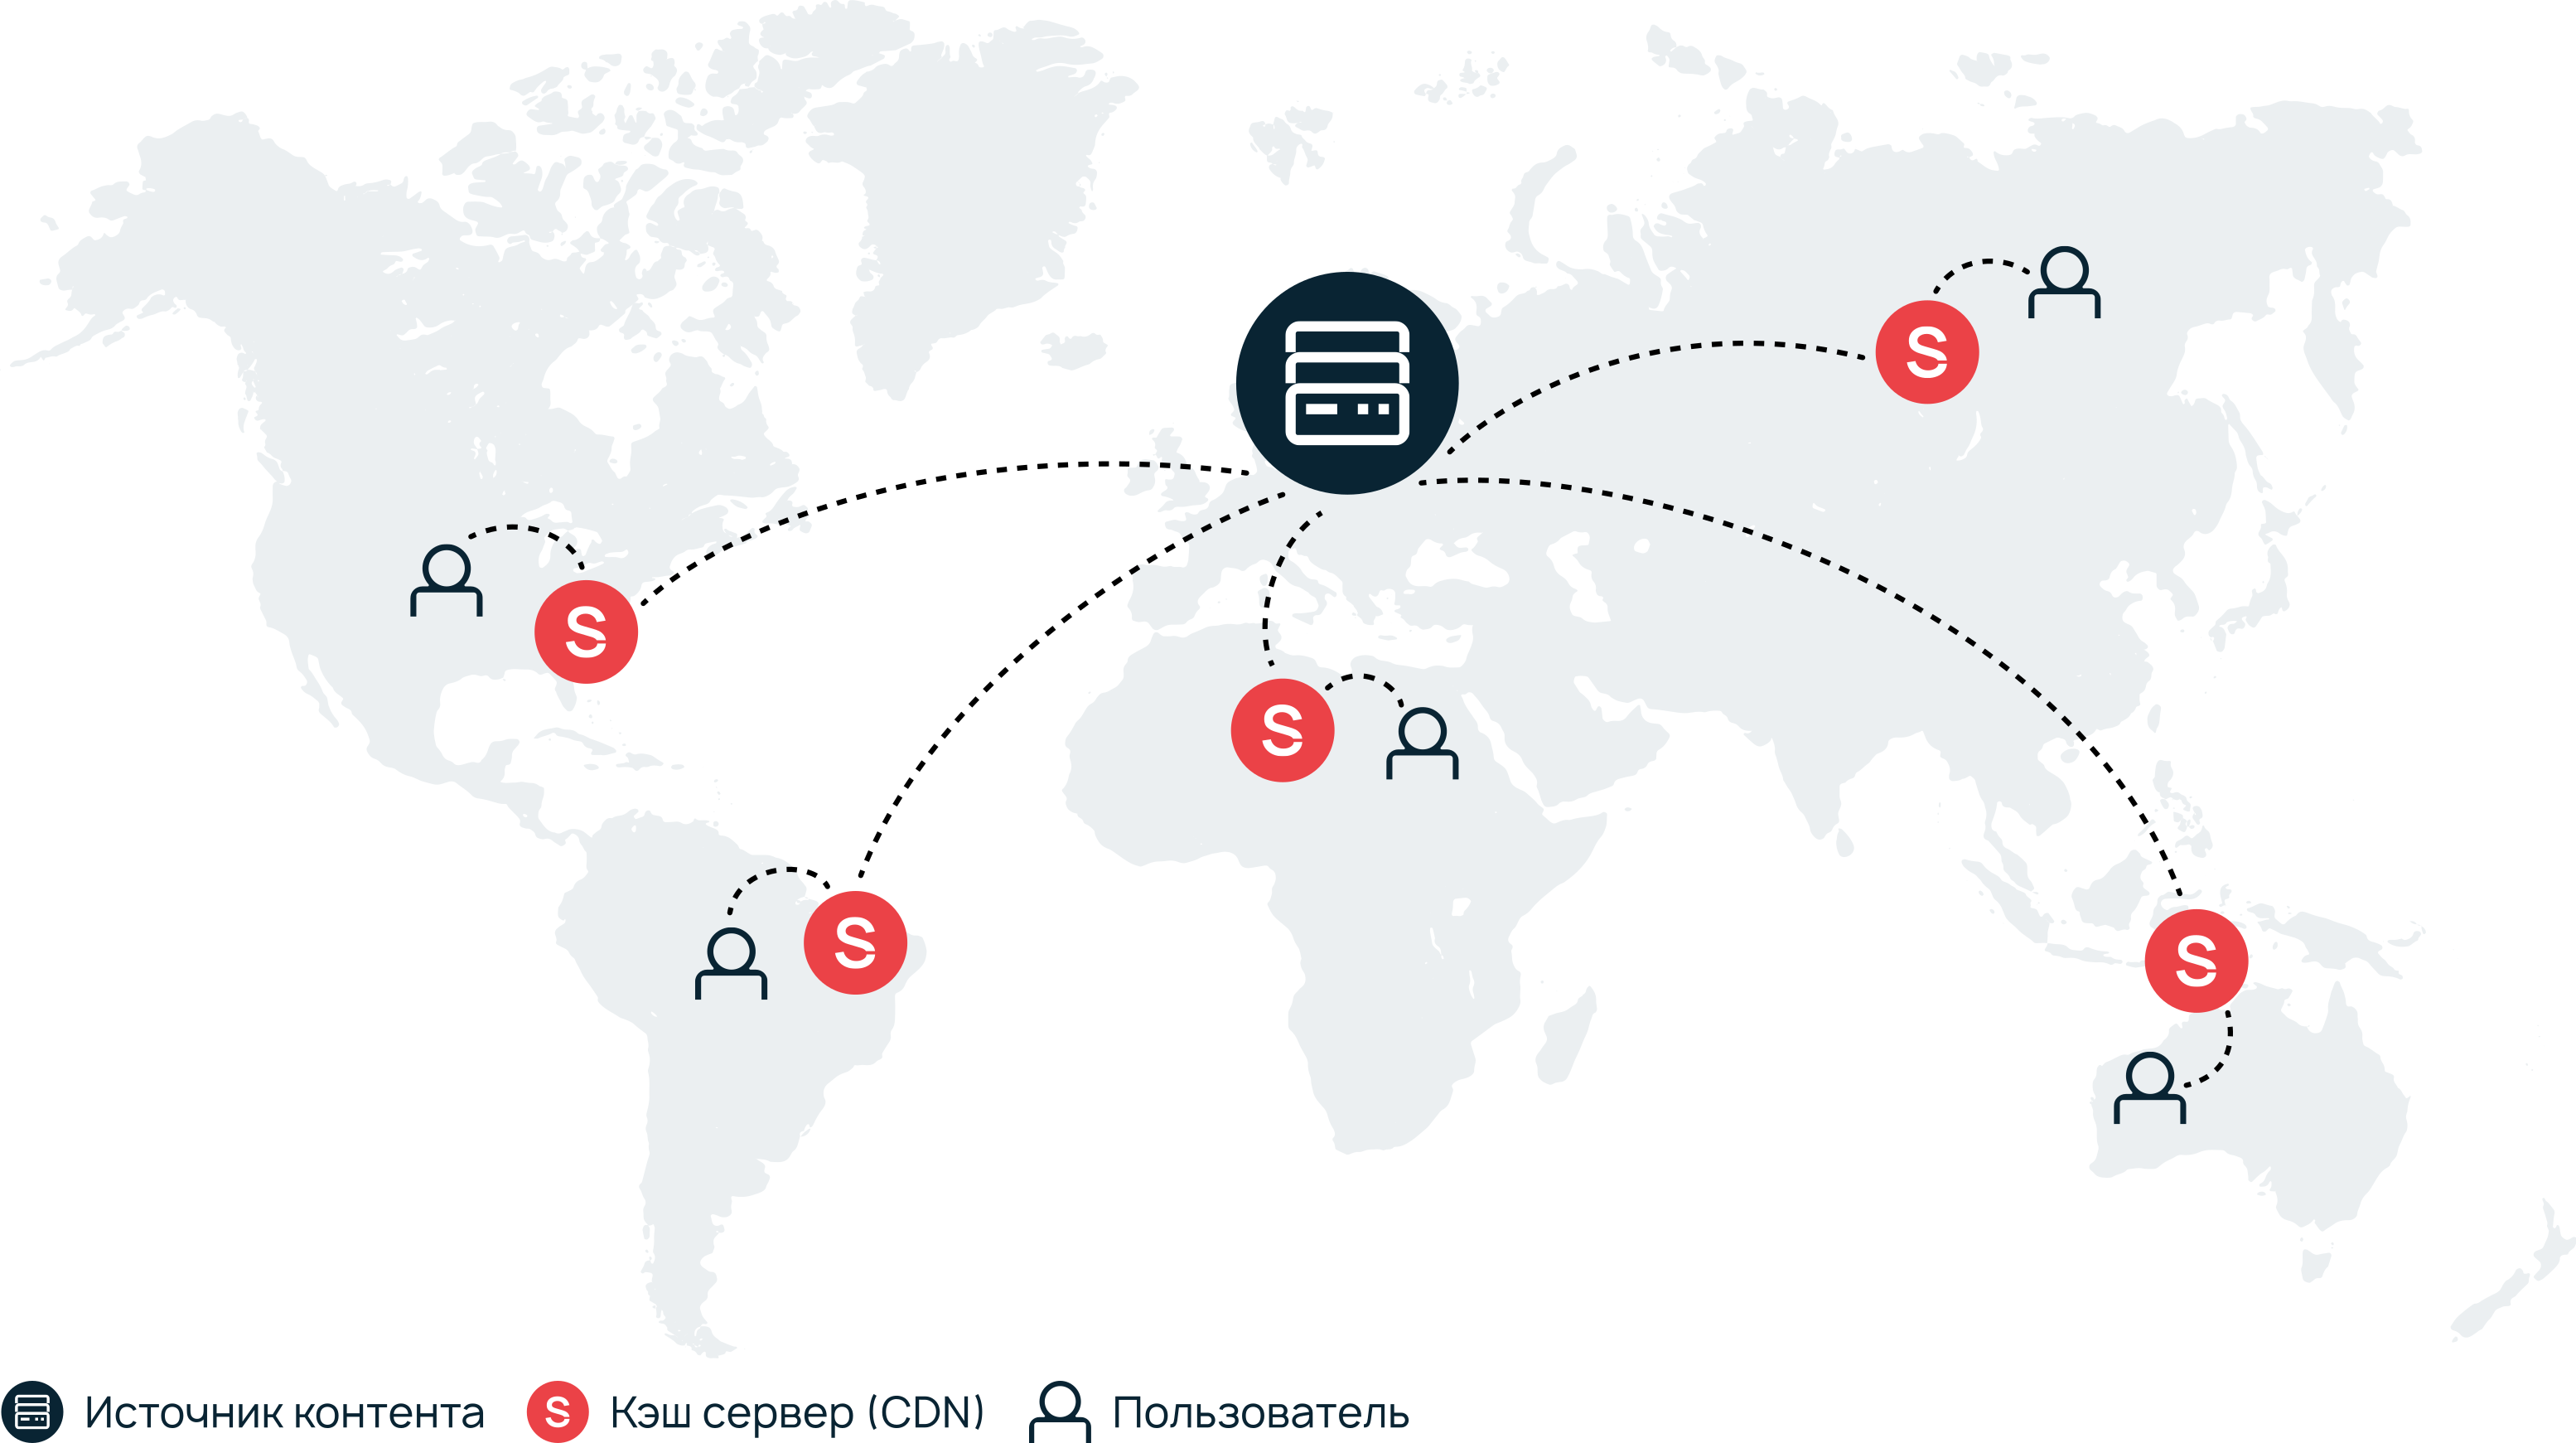
\includegraphics[width=.8\textwidth]{graphics/img/sheme-cdn}
  \caption{Пример визуализации работы CDN}
  \label{fig:mono}
\end{figure}

Когда разработчик выдает команду для установки определенного модуля, клиент обращается к своему реестру (образу базы данных всех доступных модулей), который размещен в CDN.

Работая в совокупности с CDN, система осуществляет следующие функции:

\begin{enumerate}
    \item Обеспечивает надежную и быструю доставку пакетов на компьютеры разработчиков.
    \item Снижает задержку в сети благодаря географическому размещению серверов CDN ближе к пользователям.
    \item Обеспечивает глобальное масштабирование, так как CDN может эффективно обслуживать тысячи запросов по всей России в разных частях и всему миру.
    \item Увеличивает отказоустойчивость и распределенность системы, поскольку множество точек присутствия CDN могут обслуживать запросы в случае отказа какой-либо из них.
    \item Снижает нагрузку на основные сервисы за счет кеширования.
\end{enumerate}

 При проектировании я решил воспользоваться услуги отечественного провайдера CDN компании Selectel. \cite{cdn:selectel} Данный провайдер был выбран на основании предлагаемых им услуг и их качества.

Selectel предоставляет надежные CDN-услуги, что значительно ускоряет загрузку контента, где бы пользователь не находился. Это особенно важно для нашего проекта, так как ориентир на географически распределенную аудиторию и нуждаемся в том, чтобы модули доставлялись быстро и надежно.

Компания обеспечивает высокую доступность пакетов из-за использования глобальной сети серверов внутри России и по всему миру.

При этом зона собственного покрытия CDN Selectel включает себя такие города \cite{cdn:selectel}, как:
\begin{itemize}
    \item Россия: Барнаул, Владивосток, Екатеринбург, Иркутск, Казань, Кемерово, Кизляр, Краснодар, Красноярск, Москва, Новосибирск, Орел, Ростов-на-Дону, Санкт-Петербург, Самара, Симферополь, Уфа, Хабаровск, Южно-Сахалинск
    \item Азия: Алматы, Бишкек, Гонконг, Сингапур, Ташкент
    \item Америка: Ашберн, Сан-Паулу
    \item Европа: Амстердам, Минск, Сухум, Франкфурт
\end{itemize}

\begin{figure}
  \centering
  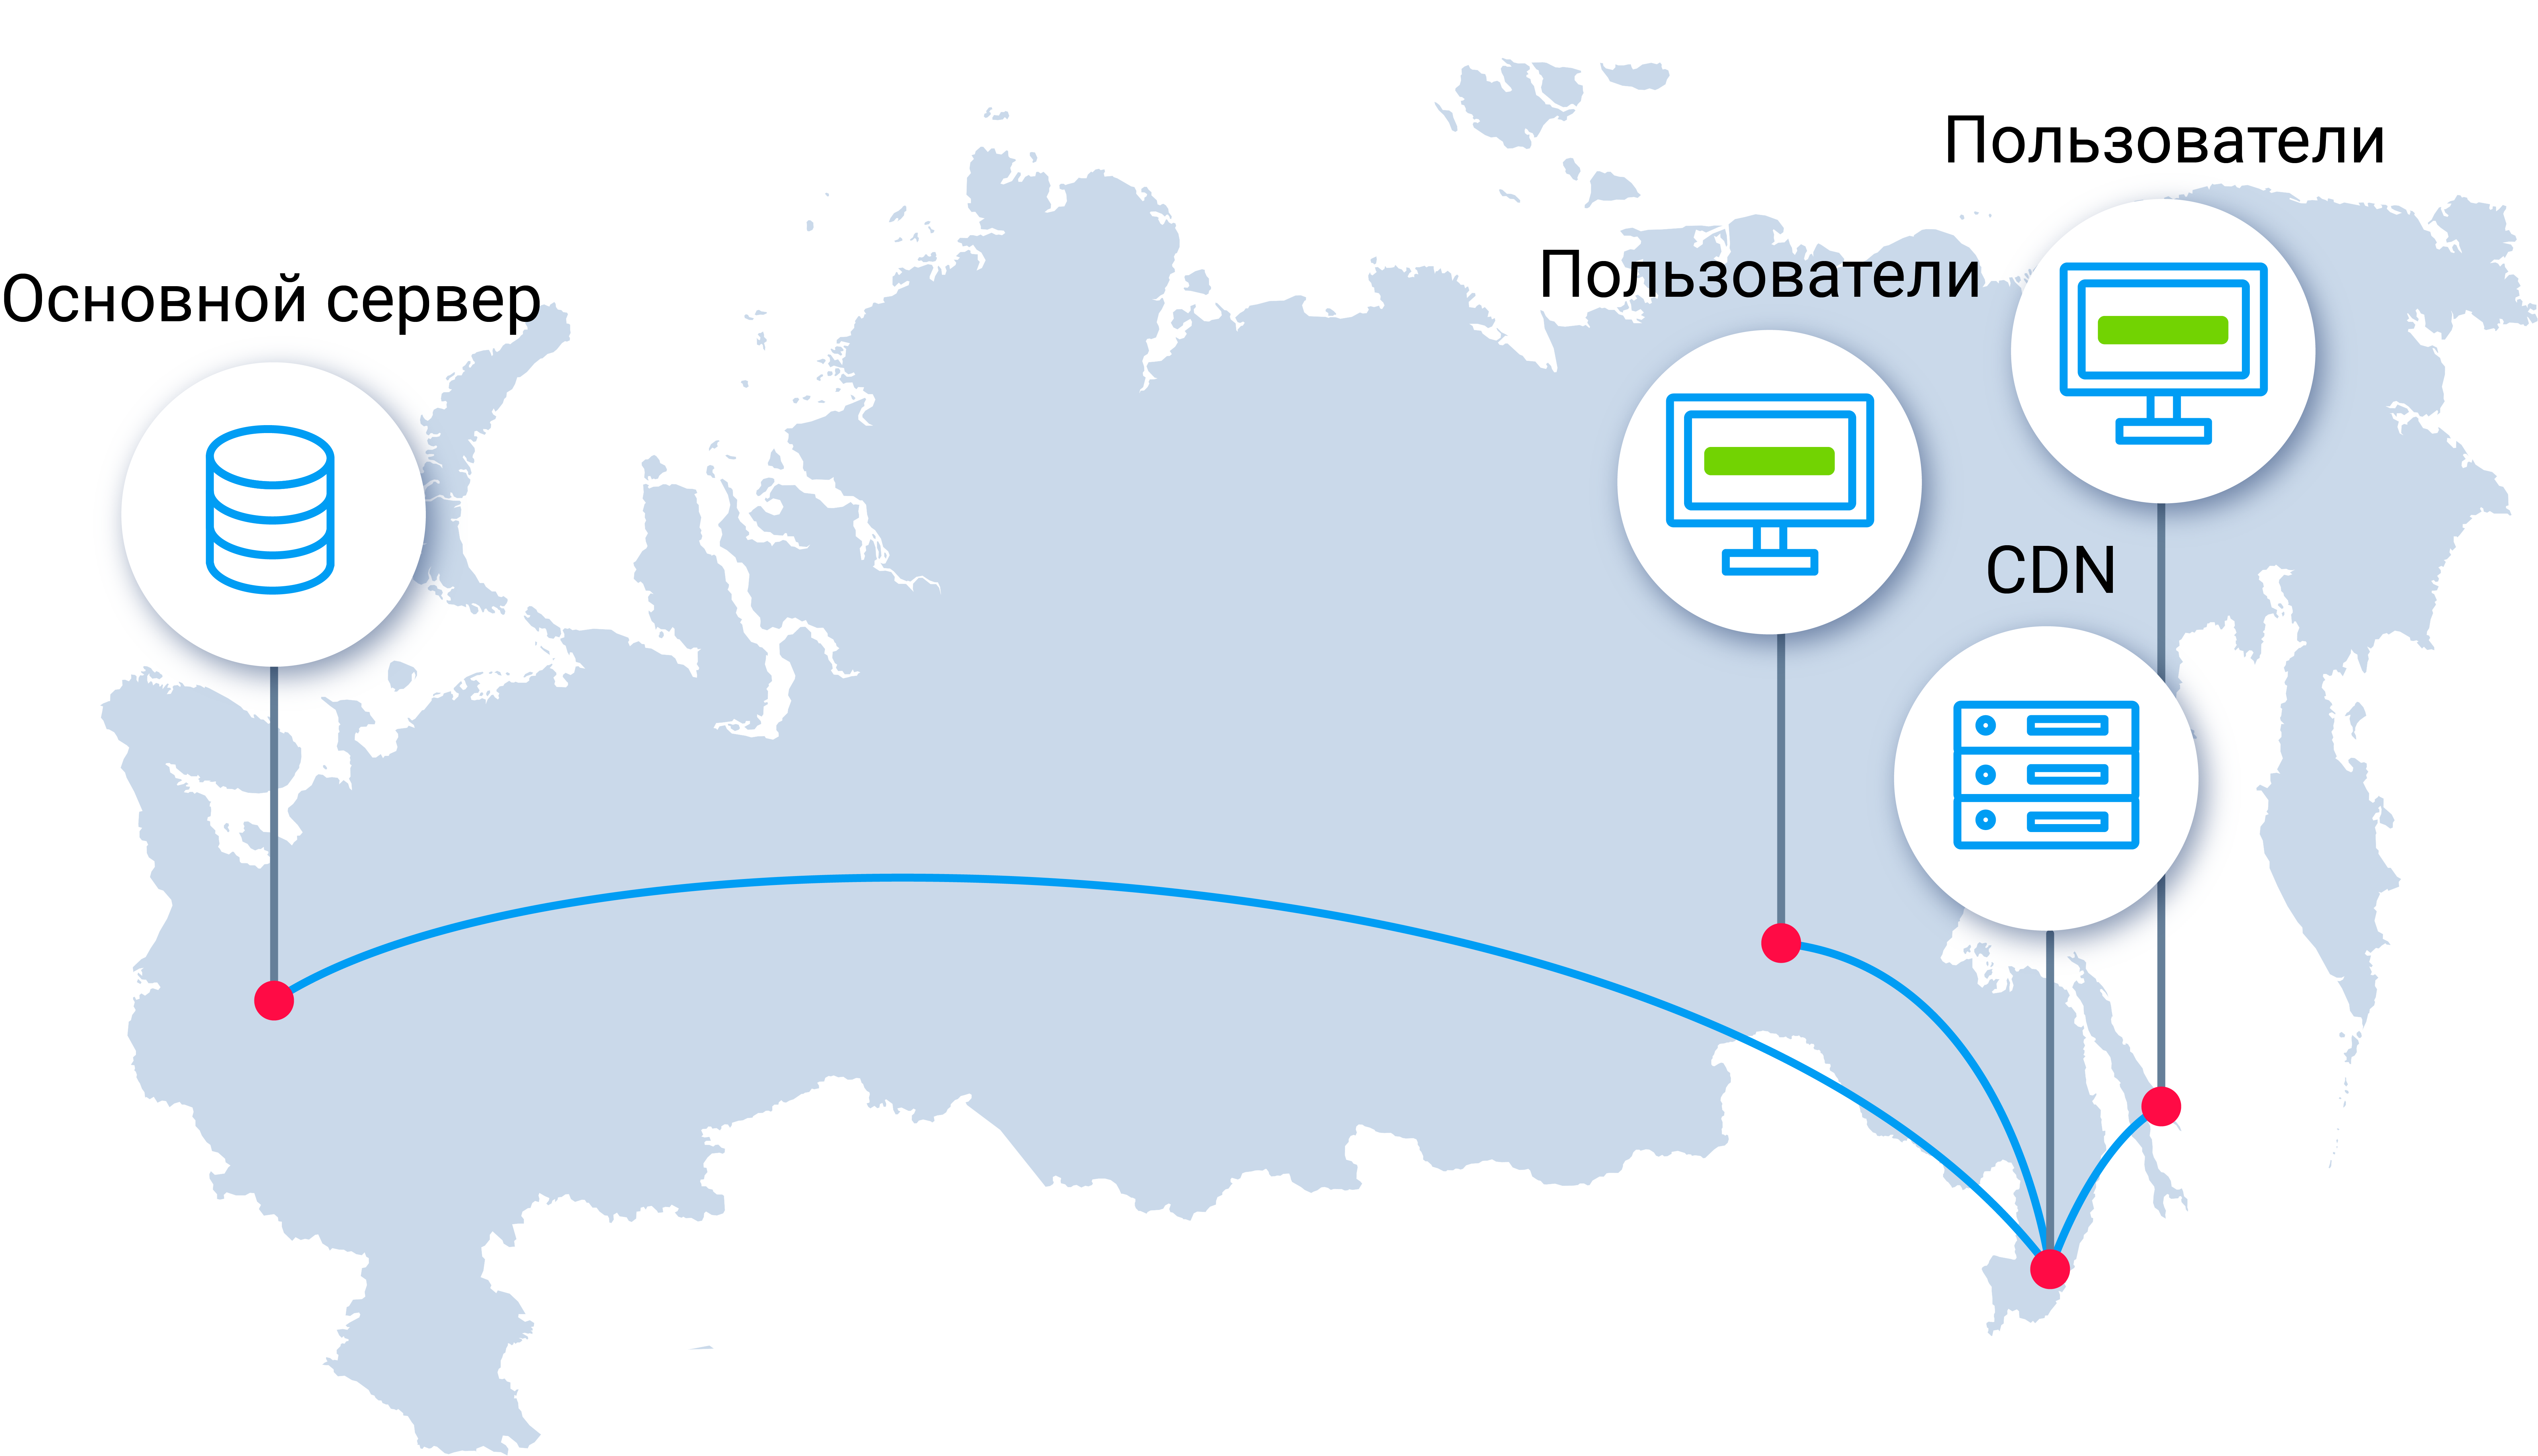
\includegraphics[width=.8\textwidth]{graphics/img/cdn.scheme.5Y4Ydf}
  \caption{Пример визуализации работы CDN в рамках России}
  \label{fig:cdn_russia}
\end{figure}

Это увеличивает отказоустойчивость проекта и позволяет нам быть уверенными в постоянной доступности модулей для пользователей.

Серверы Selectel обладают высокой пропускной способностью, что среднее время отлика составляет 30 милисекунд \cite{cdn:selectel}, обеспечивая максимальную скорость передачи данных. Это особенно ценно для системы модульного менеджера, поскольку мы имеем дело с большим количеством пакетов, которые должны быть быстро доставлены пользователям.

Кроме того, Selectel уделяет особое внимание вопросам безопасности и защиты данных. Наши пакеты и пользовательские данные хранятся с учетом последних стандартов безопасности, и мы можем быть уверенны в их надежности и защищенности.

При работе с отечественным провайдером у нас также есть возможность получить более оперативную техническую поддержку и консультации по связанным вопросам, что значительно упрощает процесс взаимодействия и решения возникающих вопросов.

В целом, CDN, как он встроен в систему, является одним из ключевых факторов обеспечения эффективной и надежной доставки пакетов и модулей. Использование услуг CDN от Selectel обеспечивает надежность и высокую скорость доставки пакетов. Кроме того, оно гарантирует высокую степень безопасности данных. Это ускоряет время развертывания и обновления проектов. При этом, такой подход снижает время простоя, что повышает общую производительность и эффективность процесса разработки ПО.

\section{Оборудование и ОС как часть системы}

Учитывая связанные риски и выработанные с этим направления, при проектировании возникает необходимость создания специального решения. Это решение должно быть совместимым с российским процессором. Данный процессор выпускает компания МЦСТ под названием «Эльбрус-8СВ» \cite{dev:elbrus_cpu}. 

Эльбрус-8СВ - является восьмиядерным промышленным процессором на базе архитектуры Эльбрус (e2k) с использованием длинного командного слова (VLIW), разработанным в России. Он создан для работы в 64-разрядной вычислительной системе и может обрабатывать до 288 гигафлопс двойной точности в одноядерном режиме при частоте 1.5 ГГц, будучи произведенным по техническим нормам в 28 нанометров. 

\Define{Гигафлопс}{Индикатор, определяющий скорость работы суперкомпьютера. 1 г= 109 aial/s, т. е. суперкомпьютер 1 сек.в 1 млрд. выполняет арифметические и логические операции.}

\Define{VLIW}{Very Long Instruction Word ""--- архитектура процессоров с несколькими вычислительными устройствами. Характеризуется тем, что одна инструкция процессора содержит несколько операций, которые должны выполняться параллельно. Фактически это «видимое программисту» микропрограммное управление, когда машинный код представляет собой лишь немного свёрнутый микрокод для непосредственного управления аппаратурой}

Ключевым преимуществом Эльбруса является его отечественное происхождение, что даёт возможность избегать определенных проблем и рисков, связанных с использованием процессоров Intel и AMD. При этом, параметры процессора позволяют полностью закрыть вопрос в потребностях сервисов.

\begin{figure}
  \centering
  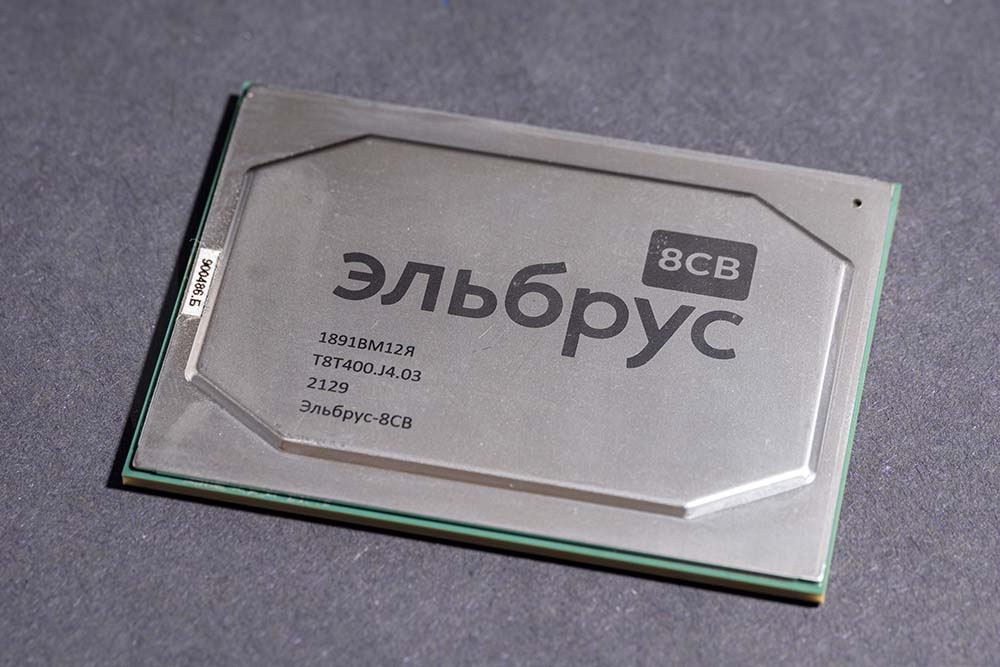
\includegraphics[width=.6\textwidth]{graphics/img/elbrus}
  \caption{Внешний вид процессора компании МЦСТ - Эльбрус-8СВ}
  \label{fig:elbrus}
\end{figure}

В 2018 году процессоры Intel, ARM, AMD и другие были поставлены под угрозу из-за обнаружения атак Spectre и Meltdown \cite{risk:spectual_hack}. Они использовали уязвимости в спекулятивной и предсказательной вычислительной системе - методах оптимизации процессора. Суть таких атак заключается в том, что процессоры заранее вырабатывают инструкции для быстрого выполнения кода, что позволяет злоумышленникам получить доступ к конфиденциальной информации через эти предварительные вычисления.

К сожалению, попытки исправить эти уязвимости столкнулись с проблемами, такими как сбои в перезагрузке и снижение производительности у некоторых пользователей, как у Intel, так и у AMD. Впоследствии обе компании выпустили обновленные патчи для решения этих проблем.

Уязвимости Intel ME позволяют злоумышленникам полностью контролировать компьютер, обходя встроенные защитные механизмы, и получать доступ ко всем его данным. Даже когда сервер выключен, взломанный Intel ME может быть использован для заражения соседнего сервера \cite{risk:intelme}. Это вызывает тревогу и подталкивает многих пользователей отказаться от использования процессоров этих компаний.

Однако, русские процессоры Эльбрус оказались неуязвимыми для таких атак. Это обусловлено их уникальной архитектурой и методами оптимизации работы процессора, отличающимися от тех, которые используются в Intel и AMD. В частности, «Эльбрус» не использует подобное спекулятивное выполнение и системы управления процессором, поэтому эти уязвимые атаки не могут быть применены \cite{risk:elbrus_no_spectre}.

\Define{Intel ME}{Intel Management Engine  (Intel ME) ""--- это встроенный модуль микроконтроллера во всех чипсетах Intel с 2006 года, который имеет полный доступ к системе, даже когда компьютер выключен или находится в спящем режиме. Его аналогом у AMD является Secure Technology (ранее известная как Secure Processor или PSP), которая также была уязвима для атак, подобных Intel ME \cite{risk:amdpsp}}

В качестве оптимальной операционной системы, которая поддерживает оборудование Эльбрус с использованием пакетного менеджера, рассматривать AstraLinux \cite{dev:astra_linux}. Это российский дистрибутив на основе Debian GNU/Linux, который нацелен на создание унифицированной, безопасной и легко управляемой операционной системы, c обеспечением высокого уровня защиты, что особенно важно при работе с критической инфраструктурой.


%%% Local Variables:
%%% mode: latex
%%% TeX-master: "rpz"
%%% End:
